% Options for packages loaded elsewhere
\PassOptionsToPackage{unicode}{hyperref}
\PassOptionsToPackage{hyphens}{url}
%
\documentclass[
]{article}
\usepackage{amsmath,amssymb}
\usepackage{lmodern}
\usepackage{ifxetex,ifluatex}
\ifnum 0\ifxetex 1\fi\ifluatex 1\fi=0 % if pdftex
  \usepackage[T1]{fontenc}
  \usepackage[utf8]{inputenc}
  \usepackage{textcomp} % provide euro and other symbols
\else % if luatex or xetex
  \usepackage{unicode-math}
  \defaultfontfeatures{Scale=MatchLowercase}
  \defaultfontfeatures[\rmfamily]{Ligatures=TeX,Scale=1}
\fi
% Use upquote if available, for straight quotes in verbatim environments
\IfFileExists{upquote.sty}{\usepackage{upquote}}{}
\IfFileExists{microtype.sty}{% use microtype if available
  \usepackage[]{microtype}
  \UseMicrotypeSet[protrusion]{basicmath} % disable protrusion for tt fonts
}{}
\makeatletter
\@ifundefined{KOMAClassName}{% if non-KOMA class
  \IfFileExists{parskip.sty}{%
    \usepackage{parskip}
  }{% else
    \setlength{\parindent}{0pt}
    \setlength{\parskip}{6pt plus 2pt minus 1pt}}
}{% if KOMA class
  \KOMAoptions{parskip=half}}
\makeatother
\usepackage{xcolor}
\IfFileExists{xurl.sty}{\usepackage{xurl}}{} % add URL line breaks if available
\IfFileExists{bookmark.sty}{\usepackage{bookmark}}{\usepackage{hyperref}}
\hypersetup{
  hidelinks,
  pdfcreator={LaTeX via pandoc}}
\urlstyle{same} % disable monospaced font for URLs
\usepackage[margin=1in]{geometry}
\usepackage{longtable,booktabs,array}
\usepackage{calc} % for calculating minipage widths
% Correct order of tables after \paragraph or \subparagraph
\usepackage{etoolbox}
\makeatletter
\patchcmd\longtable{\par}{\if@noskipsec\mbox{}\fi\par}{}{}
\makeatother
% Allow footnotes in longtable head/foot
\IfFileExists{footnotehyper.sty}{\usepackage{footnotehyper}}{\usepackage{footnote}}
\makesavenoteenv{longtable}
\usepackage{graphicx}
\makeatletter
\def\maxwidth{\ifdim\Gin@nat@width>\linewidth\linewidth\else\Gin@nat@width\fi}
\def\maxheight{\ifdim\Gin@nat@height>\textheight\textheight\else\Gin@nat@height\fi}
\makeatother
% Scale images if necessary, so that they will not overflow the page
% margins by default, and it is still possible to overwrite the defaults
% using explicit options in \includegraphics[width, height, ...]{}
\setkeys{Gin}{width=\maxwidth,height=\maxheight,keepaspectratio}
% Set default figure placement to htbp
\makeatletter
\def\fps@figure{htbp}
\makeatother
\setlength{\emergencystretch}{3em} % prevent overfull lines
\providecommand{\tightlist}{%
  \setlength{\itemsep}{0pt}\setlength{\parskip}{0pt}}
\setcounter{secnumdepth}{5}
\ifluatex
  \usepackage{selnolig}  % disable illegal ligatures
\fi

\author{}
\date{\vspace{-2.5em}}

\begin{document}

{
\setcounter{tocdepth}{2}
\tableofcontents
}
\newcommand{\studyname}{mock}

\newcommand{\pathCoRoutput}{cor_coxph/output/D57}

\hypertarget{cor-coxph}{%
\section{Day 57 Univariate CoR: Cox Models of Risk}\label{cor-coxph}}

The main regression model is the Cox proportional hazards model. All plots are made with Cox models fit unless specified otherwise.

\hypertarget{hazard-ratios}{%
\subsection{Hazard ratios}\label{hazard-ratios}}

\begin{table}[H]
\caption{Inference for Day 57 antibody marker covariate-adjusted correlates of risk of COVID in the vaccine group: Hazard ratios per 10-fold increment in the marker*}
\begin{center}
    \begin{tabular}{lcccccc}
   \hline
 
         \multicolumn{1}{l}{Mock} & \multicolumn{1}{c}{No. cases /}   & \multicolumn{2}{c}{HR per 10-fold incr.}                     & \multicolumn{1}{c}{P-value}   & \multicolumn{1}{c}{q-value}   & \multicolumn{1}{c}{FWER} \\ 
         \multicolumn{1}{l}{Immunologic Marker}            & \multicolumn{1}{c}{No. at-risk**} & \multicolumn{1}{c}{Pt. Est.} & \multicolumn{1}{c}{95\% CI} & \multicolumn{1}{c}{(2-sided)} & \multicolumn{1}{c}{} & \multicolumn{1}{c}{} \\ 
         \hline
 
            
 \multicolumn{5}{l}{Day 57} \\ 
Anti Spike IgG (IU/ml) & 71/13,295 & 0.11 & (0.07-0.18) & $<$0.001 & $<$0.001 & $<$0.001 \\ 
  Anti RBD IgG (IU/ml) & 71/13,295 & 0.31 & (0.23-0.42) & $<$0.001 & $<$0.001 & $<$0.001 \\ 
  Pseudovirus-nAb ID50 & 71/13,295 & 0.36 & (0.27-0.50) & $<$0.001 & $<$0.001 & $<$0.001 \\ 
  Pseudovirus-nAb ID80 & 71/13,295 & 0.45 & (0.33-0.60) & $<$0.001 & $<$0.001 & $<$0.001 \\ 
          
 \multicolumn{5}{l}{} \\ 
        
 \multicolumn{5}{l}{Fold-rise} \\ 
Anti Spike IgG (IU/ml) & 71/13,295 & 0.10 & (0.05-0.17) & $<$0.001 & $<$0.001 & $<$0.001 \\ 
  Anti RBD IgG (IU/ml) & 71/13,295 & 0.34 & (0.25-0.46) & $<$0.001 & $<$0.001 & $<$0.001 \\ 
  Pseudovirus-nAb ID50 & 71/13,295 & 0.48 & (0.36-0.64) & $<$0.001 & $<$0.001 & $<$0.001 \\ 
  Pseudovirus-nAb ID80 & 71/13,295 & 0.43 & (0.32-0.58) & $<$0.001 & $<$0.001 & $<$0.001 \\ 
   \hline
\end{tabular}
\\
\end{center}
*Baseline covariates adjusted for: age in years, at risk or not, community of color or not
%, baseline risk score
. Average follow-up time \input{cor_coxph/output/D57/CoR_mean_followup_time_vacc_mock} days, maximum follow-up time \input{cor_coxph/output/D57/CoR_max_followup_time_vacc_mock} days.\\
**No. at-risk = number of per-protocol baseline negative vaccine recipients at-risk for COVID at 7 days post Day 57 visit; no. cases = number of this cohort with an observed COVID endpoints.

    \label{tab:CoR_univariable_svycoxph_pretty_mock}
\end{table}

\begin{table}[H]
\caption{Inference for Day 57 antibody marker covariate-adjusted correlates of risk of COVID in the vaccine group: Hazard ratios for Middle vs. Upper tertile vs. Lower tertile*}
\begin{center}
\setlength{\tabcolsep}{.5ex}
\begin{tabular}{lccccccccc}
   \hline
 
         \multicolumn{1}{l}{Mock} & \multicolumn{1}{c}{Tertile}   & \multicolumn{1}{c}{No. cases /}   & \multicolumn{1}{c}{Attack}   & \multicolumn{2}{c}{HR per 10-fold incr.}                     & \multicolumn{1}{c}{P-value}   & \multicolumn{1}{c}{Overall P-}      & \multicolumn{1}{c}{Overall q-}   & \multicolumn{1}{c}{Overall} \\ 
         \multicolumn{1}{l}{Immunologic Marker}            & \multicolumn{1}{c}{}          & \multicolumn{1}{c}{No. at-risk**} & \multicolumn{1}{c}{rate}   & \multicolumn{1}{c}{Pt. Est.} & \multicolumn{1}{c}{95\% CI} & \multicolumn{1}{c}{(2-sided)} & \multicolumn{1}{c}{value***} & \multicolumn{1}{c}{value} & \multicolumn{1}{c}{FWER} \\ 
         \hline
 
            
 \multicolumn{8}{l}{Day 57} \\ 
Anti Spike IgG & Lower & 66/4,430 & 0.0149 & 1 & N/A & N/A & $<$0.001 & $<$0.001 & $<$0.001 \\ 
  (IU/ml) & Middle & 4/4,412 & 0.0009 & 0.07 & (0.02-0.20) & $<$0.001 &     &     &     \\ 
   & Upper & 1/4,456 & 0.0002 & 0.01 & (0.00-0.06) & $<$0.001 &     &     &     \\ 
  Anti RBD IgG & Lower & 47/4,430 & 0.0106 & 1 & N/A & N/A & $<$0.001 & $<$0.001 & $<$0.001 \\ 
  (IU/ml) & Middle & 17/4,432 & 0.0038 & 0.46 & (0.23-0.90) & 0.023 &     &     &     \\ 
   & Upper & 7/4,435 & 0.0016 & 0.10 & (0.04-0.23) & $<$0.001 &     &     &     \\ 
  Pseudovirus-nAb & Lower & 48/4,424 & 0.0108 & 1 & N/A & N/A & $<$0.001 & $<$0.001 & $<$0.001 \\ 
  ID50 & Middle & 16/4,440 & 0.0036 & 0.31 & (0.16-0.61) & 0.001 &     &     &     \\ 
   & Upper & 7/4,433 & 0.0016 & 0.11 & (0.05-0.27) & $<$0.001 &     &     &     \\ 
  Pseudovirus-nAb & Lower & 57/4,431 & 0.0129 & 1 & N/A & N/A & $<$0.001 & $<$0.001 & $<$0.001 \\ 
  ID80 & Middle & 11/4,426 & 0.0025 & 0.22 & (0.11-0.44) & $<$0.001 &     &     &     \\ 
   & Upper & 3/4,440 & 0.0007 & 0.04 & (0.01-0.14) & $<$0.001 &     &     &     \\ 
          
 \multicolumn{8}{l}{} \\ 
        
 \multicolumn{8}{l}{Fold-rise} \\ 
Anti Spike IgG & Lower & 63/4,429 & 0.0142 & 1 & N/A & N/A & $<$0.001 & $<$0.001 & $<$0.001 \\ 
  (IU/ml) & Middle & 7/4,435 & 0.0016 & 0.13 & (0.06-0.31) & $<$0.001 &     &     &     \\ 
   & Upper & 1/4,433 & 0.0002 & 0.01 & (0.00-0.05) & $<$0.001 &     &     &     \\ 
  Anti RBD IgG & Lower & 49/4,437 & 0.0110 & 1 & N/A & N/A & $<$0.001 & $<$0.001 & $<$0.001 \\ 
  (IU/ml) & Middle & 19/4,437 & 0.0043 & 0.32 & (0.17-0.59) & $<$0.001 &     &     &     \\ 
   & Upper & 3/4,424 & 0.0007 & 0.03 & (0.01-0.12) & $<$0.001 &     &     &     \\ 
  Pseudovirus-nAb & Lower & 49/4,460 & 0.0110 & 1 & N/A & N/A & $<$0.001 & $<$0.001 & $<$0.001 \\ 
  ID50 & Middle & 13/4,438 & 0.0029 & 0.31 & (0.15-0.62) & 0.001 &     &     &     \\ 
   & Upper & 9/4,400 & 0.0020 & 0.16 & (0.07-0.36) & $<$0.001 &     &     &     \\ 
  Pseudovirus-nAb & Lower & 52/4,432 & 0.0117 & 1 & N/A & N/A & $<$0.001 & $<$0.001 & $<$0.001 \\ 
  ID80 & Middle & 16/4,410 & 0.0036 & 0.30 & (0.16-0.56) & $<$0.001 &     &     &     \\ 
   & Upper & 3/4,455 & 0.0007 & 0.05 & (0.01-0.17) & $<$0.001 &     &     &     \\ 
    
 \multicolumn{8}{l}{} \\ 

 \multicolumn{2}{l}{Placebo} & 710/13,326&0.0533&\multicolumn{4}{l}{}  \\ 
 \hline
\end{tabular}
\\
\end{center}
*Baseline covariates adjusted for: age in years, at risk or not, community of color or not
%, baseline risk score
. Average follow-up time \input{cor_coxph/output/D57/CoR_mean_followup_time_vacc_mock} days, maximum follow-up time \input{cor_coxph/output/D57/CoR_max_followup_time_vacc_mock} days. 
Cutpoints: 
%Day 57 cutpoints: 
\input{cor_coxph/output/D57/cutpoints_D57bindSpike_mock},  
\input{cor_coxph/output/D57/cutpoints_D57bindRBD_mock},  
\input{cor_coxph/output/D57/cutpoints_D57pseudoneutid50_mock},  
\input{cor_coxph/output/D57/cutpoints_D57pseudoneutid80_mock}.
%fold-rise cutpoints: 
%\input{\pathCoRoutput/cutpoints_D57overBbindSpike_\studyname},  
%\input{\pathCoRoutput/cutpoints_D57overBbindRBD_\studyname},  
%\input{\pathCoRoutput/cutpoints_D57overBpseudoneutid50_\studyname},  
%\input{\pathCoRoutput/cutpoints_D57overBpseudoneutid80_\studyname}.  
\\
**No. at-risk = number of per-protocol baseline negative vaccine recipients at-risk for COVID at 7 days post Day 57 visit; no. cases = number of this cohort with an observed COVID endpoints.\\
***Generalized Wald-test p-value of the null hypothesis that the hazard rate is constant across the Lower, Middle, and Upper tertile groups.

    \label{tab:CoR_univariable_svycoxph_cat_pretty_mock}
\end{table}

\begin{figure}[H]
    \includegraphics[width=1\textwidth]{cor_coxph/output/D57/hr_forest_bindSpike_mock}
    \includegraphics[width=1\textwidth]{cor_coxph/output/D57/hr_forest_bindRBD_mock}
    \includegraphics[width=1\textwidth]{cor_coxph/output/D57/hr_forest_pseudoneutid50_mock}
    \includegraphics[width=1\textwidth]{cor_coxph/output/D57/hr_forest_pseudoneutid80_mock}
    \caption{Forest plots of hazard ratios among baseline seronegative vaccine recipients and subgroups with 95\% point-wise confidence intervals.}
\end{figure}

\clearpage

\begin{figure}[H]
    \centering
    \includegraphics[width=1\textwidth]{cor_coxph/output/D57/hr_forest_marginal_bindSpike_mock}
    \caption{Forest plots of hazard ratios of Day 57 binding Ab to spike markers among baseline seronegative vaccine recipients (top row) and eight subpopulations (row 2-9) with 95\% point-wise confidence intervals.}
\end{figure}

\begin{figure}[H]
    \centering
    \includegraphics[width=1\textwidth]{cor_coxph/output/D57/hr_forest_marginal_bindRBD_mock}
    \caption{Forest plots of hazard ratios of Day 57 binding Ab to RBD markers among baseline seronegative vaccine recipients (top row) and eight subpopulations (row 2-9) with 95\% point-wise confidence intervals.}
\end{figure}

\begin{figure}[H]
    \centering
    \includegraphics[width=1\textwidth]{cor_coxph/output/D57/hr_forest_marginal_pseudoneutid50_mock}
    \caption{Forest plots of hazard ratios of Day 57 pseudo neut ID50 markers among baseline seronegative vaccine recipients (top row) and eight subpopulations (row 2-9) with 95\% point-wise confidence intervals.}
\end{figure}

\begin{figure}[H]
    \centering
    \includegraphics[width=1\textwidth]{cor_coxph/output/D57/hr_forest_marginal_pseudoneutid80_mock}
    \caption{Forest plots of hazard ratios of Day 57 pseudo neut ID80 markers among baseline seronegative vaccine recipients (top row) and eight subpopulations (row 2-9) with 95\% point-wise confidence intervals.}
\end{figure}

\clearpage

\hypertarget{marginalized-risk-and-controlled-vaccine-efficacy-plots}{%
\subsection{Marginalized risk and controlled vaccine efficacy plots}\label{marginalized-risk-and-controlled-vaccine-efficacy-plots}}

\begin{figure}[H]
    \centering
    \includegraphics[width=1\textwidth]{cor_coxph/output/D57/marginalized_risks1_mock}
    \caption{Marginalized cumulative risk by Day \protect\input{cor_coxph/output/D57/timepoints_cum_risk_mock} as functions of Day 57 markers (=s) among baseline seronegative vaccine recipients with 95\% bootstrap point-wise confidence bands. The horizontal lines indicate the overall cumulative risk of the placebo and vaccine arms by Day \protect\input{cor_coxph/output/D57/timepoints_cum_risk_mock} and its 95\% point-wise confidence interval. Histograms of the immunological markers in the vaccine arm are overlaid. lod: lower limit of detection.}
\end{figure}

\begin{figure}[H]
    \centering
    \includegraphics[width=1\textwidth]{cor_coxph/output/D57/marginalized_risks2_woplacebo_mock}
    \caption{Marginalized cumulative risk by Day \protect\input{cor_coxph/output/D57/timepoints_cum_risk_mock} as functions of Day 57 markers above a threshold ($\geq s$) among baseline seronegative vaccine recipients with 95\% bootstrap point-wise confidence bands (at least 5 cases are required). The horizontal lines indicate the overall cumulative risk of the vaccine arm by Day \protect\input{cor_coxph/output/D57/timepoints_cum_risk_mock} and its 95\% point-wise confidence interval. Histograms of the immunological markers in the vaccine arm are overlaid. lod: lower limit of detection.}
\end{figure}

\begin{figure}[H]
    \centering
    \includegraphics[width=1\textwidth]{cor_coxph/output/D57/controlled_ve_curves_mock}
    \caption{Controlled VE with sensitivity analysis as functions of Day 57 markers (=s) among baseline seronegative vaccine recipients with 95\% bootstrap point-wise confidence bands. Histograms of the immunological markers in the vaccine arm are overlaid. lod: lower limit of detection.}
\end{figure}

\begin{figure}[H]
    \centering
    \includegraphics[width=1\textwidth]{cor_coxph/output/D57/marginalized_risks_cat_mock}
    \caption{Marginalized cumulative incidence rate curves for trichotomized Day 57 markers among baseline seronegative vaccine recipients. The gray line is the overall cumulative incidence rate curve in the placebo arm.}
\end{figure}

\clearpage

\renewcommand{\pathCoRoutput}{cor_coxph/output/D29}

\hypertarget{cor-coxph}{%
\section{Day 29 Univariate CoR: Cox Models of Risk}\label{cor-coxph}}

The main regression model is the Cox proportional hazards model. All plots are made with Cox models fit unless specified otherwise.

\hypertarget{hazard-ratios-1}{%
\subsection{Hazard ratios}\label{hazard-ratios-1}}

\begin{table}[H]
\caption{Inference for Day 29 antibody marker covariate-adjusted correlates of risk of COVID in the vaccine group: Hazard ratios per 10-fold increment in the marker*}
\begin{center}
    \begin{tabular}{lcccccc}
   \hline
 
         \multicolumn{1}{l}{Mock} & \multicolumn{1}{c}{No. cases /}   & \multicolumn{2}{c}{HR per 10-fold incr.}                     & \multicolumn{1}{c}{P-value}   & \multicolumn{1}{c}{q-value}   & \multicolumn{1}{c}{FWER} \\ 
         \multicolumn{1}{l}{Immunologic Marker}            & \multicolumn{1}{c}{No. at-risk**} & \multicolumn{1}{c}{Pt. Est.} & \multicolumn{1}{c}{95\% CI} & \multicolumn{1}{c}{(2-sided)} & \multicolumn{1}{c}{} & \multicolumn{1}{c}{} \\ 
         \hline
 
            
 \multicolumn{5}{l}{Day 57} \\ 
Anti Spike IgG (IU/ml) & 71/13,295 & 0.11 & (0.07-0.18) & $<$0.001 & $<$0.001 & $<$0.001 \\ 
  Anti RBD IgG (IU/ml) & 71/13,295 & 0.31 & (0.23-0.42) & $<$0.001 & $<$0.001 & $<$0.001 \\ 
  Pseudovirus-nAb ID50 & 71/13,295 & 0.36 & (0.27-0.50) & $<$0.001 & $<$0.001 & $<$0.001 \\ 
  Pseudovirus-nAb ID80 & 71/13,295 & 0.45 & (0.33-0.60) & $<$0.001 & $<$0.001 & $<$0.001 \\ 
          
 \multicolumn{5}{l}{} \\ 
        
 \multicolumn{5}{l}{Fold-rise} \\ 
Anti Spike IgG (IU/ml) & 71/13,295 & 0.10 & (0.05-0.17) & $<$0.001 & $<$0.001 & $<$0.001 \\ 
  Anti RBD IgG (IU/ml) & 71/13,295 & 0.34 & (0.25-0.46) & $<$0.001 & $<$0.001 & $<$0.001 \\ 
  Pseudovirus-nAb ID50 & 71/13,295 & 0.48 & (0.36-0.64) & $<$0.001 & $<$0.001 & $<$0.001 \\ 
  Pseudovirus-nAb ID80 & 71/13,295 & 0.43 & (0.32-0.58) & $<$0.001 & $<$0.001 & $<$0.001 \\ 
   \hline
\end{tabular}
\\
\end{center}
*Baseline covariates adjusted for: age in years, at risk or not, community of color or not
%, baseline risk score
. Average follow-up time \input{cor_coxph/output/D29/CoR_mean_followup_time_vacc_mock} days, maximum follow-up time \input{cor_coxph/output/D29/CoR_max_followup_time_vacc_mock} days.\\
**No. at-risk = number of per-protocol baseline negative vaccine recipients at-risk for COVID at 7 days post Day 29 visit; no. cases = number of this cohort with an observed COVID endpoints.

    \label{tab:CoR_univariable_svycoxph_pretty_mock}
\end{table}

\begin{table}[H]
\caption{Inference for Day 29 antibody marker covariate-adjusted correlates of risk of COVID in the vaccine group: Hazard ratios for Middle vs. Upper tertile vs. Lower tertile*}
\begin{center}
\setlength{\tabcolsep}{.5ex}
\begin{tabular}{lccccccccc}
   \hline
 
         \multicolumn{1}{l}{Mock} & \multicolumn{1}{c}{Tertile}   & \multicolumn{1}{c}{No. cases /}   & \multicolumn{1}{c}{Attack}   & \multicolumn{2}{c}{HR per 10-fold incr.}                     & \multicolumn{1}{c}{P-value}   & \multicolumn{1}{c}{Overall P-}      & \multicolumn{1}{c}{Overall q-}   & \multicolumn{1}{c}{Overall} \\ 
         \multicolumn{1}{l}{Immunologic Marker}            & \multicolumn{1}{c}{}          & \multicolumn{1}{c}{No. at-risk**} & \multicolumn{1}{c}{rate}   & \multicolumn{1}{c}{Pt. Est.} & \multicolumn{1}{c}{95\% CI} & \multicolumn{1}{c}{(2-sided)} & \multicolumn{1}{c}{value***} & \multicolumn{1}{c}{value} & \multicolumn{1}{c}{FWER} \\ 
         \hline
 
            
 \multicolumn{8}{l}{Day 57} \\ 
Anti Spike IgG & Lower & 66/4,430 & 0.0149 & 1 & N/A & N/A & $<$0.001 & $<$0.001 & $<$0.001 \\ 
  (IU/ml) & Middle & 4/4,412 & 0.0009 & 0.07 & (0.02-0.20) & $<$0.001 &     &     &     \\ 
   & Upper & 1/4,456 & 0.0002 & 0.01 & (0.00-0.06) & $<$0.001 &     &     &     \\ 
  Anti RBD IgG & Lower & 47/4,430 & 0.0106 & 1 & N/A & N/A & $<$0.001 & $<$0.001 & $<$0.001 \\ 
  (IU/ml) & Middle & 17/4,432 & 0.0038 & 0.46 & (0.23-0.90) & 0.023 &     &     &     \\ 
   & Upper & 7/4,435 & 0.0016 & 0.10 & (0.04-0.23) & $<$0.001 &     &     &     \\ 
  Pseudovirus-nAb & Lower & 48/4,424 & 0.0108 & 1 & N/A & N/A & $<$0.001 & $<$0.001 & $<$0.001 \\ 
  ID50 & Middle & 16/4,440 & 0.0036 & 0.31 & (0.16-0.61) & 0.001 &     &     &     \\ 
   & Upper & 7/4,433 & 0.0016 & 0.11 & (0.05-0.27) & $<$0.001 &     &     &     \\ 
  Pseudovirus-nAb & Lower & 57/4,431 & 0.0129 & 1 & N/A & N/A & $<$0.001 & $<$0.001 & $<$0.001 \\ 
  ID80 & Middle & 11/4,426 & 0.0025 & 0.22 & (0.11-0.44) & $<$0.001 &     &     &     \\ 
   & Upper & 3/4,440 & 0.0007 & 0.04 & (0.01-0.14) & $<$0.001 &     &     &     \\ 
          
 \multicolumn{8}{l}{} \\ 
        
 \multicolumn{8}{l}{Fold-rise} \\ 
Anti Spike IgG & Lower & 63/4,429 & 0.0142 & 1 & N/A & N/A & $<$0.001 & $<$0.001 & $<$0.001 \\ 
  (IU/ml) & Middle & 7/4,435 & 0.0016 & 0.13 & (0.06-0.31) & $<$0.001 &     &     &     \\ 
   & Upper & 1/4,433 & 0.0002 & 0.01 & (0.00-0.05) & $<$0.001 &     &     &     \\ 
  Anti RBD IgG & Lower & 49/4,437 & 0.0110 & 1 & N/A & N/A & $<$0.001 & $<$0.001 & $<$0.001 \\ 
  (IU/ml) & Middle & 19/4,437 & 0.0043 & 0.32 & (0.17-0.59) & $<$0.001 &     &     &     \\ 
   & Upper & 3/4,424 & 0.0007 & 0.03 & (0.01-0.12) & $<$0.001 &     &     &     \\ 
  Pseudovirus-nAb & Lower & 49/4,460 & 0.0110 & 1 & N/A & N/A & $<$0.001 & $<$0.001 & $<$0.001 \\ 
  ID50 & Middle & 13/4,438 & 0.0029 & 0.31 & (0.15-0.62) & 0.001 &     &     &     \\ 
   & Upper & 9/4,400 & 0.0020 & 0.16 & (0.07-0.36) & $<$0.001 &     &     &     \\ 
  Pseudovirus-nAb & Lower & 52/4,432 & 0.0117 & 1 & N/A & N/A & $<$0.001 & $<$0.001 & $<$0.001 \\ 
  ID80 & Middle & 16/4,410 & 0.0036 & 0.30 & (0.16-0.56) & $<$0.001 &     &     &     \\ 
   & Upper & 3/4,455 & 0.0007 & 0.05 & (0.01-0.17) & $<$0.001 &     &     &     \\ 
    
 \multicolumn{8}{l}{} \\ 

 \multicolumn{2}{l}{Placebo} & 710/13,326&0.0533&\multicolumn{4}{l}{}  \\ 
 \hline
\end{tabular}
\\
\end{center}
*Baseline covariates adjusted for: age in years, at risk or not, community of color or not
%, baseline risk score
. Average follow-up time \input{cor_coxph/output/D29/CoR_mean_followup_time_vacc_mock} days, maximum follow-up time \input{cor_coxph/output/D29/CoR_max_followup_time_vacc_mock} days. 
Cutpoints: 
%Day 29 cutpoints: 
\input{cor_coxph/output/D29/cutpoints_D29bindSpike_mock},  
\input{cor_coxph/output/D29/cutpoints_D29bindRBD_mock},  
\input{cor_coxph/output/D29/cutpoints_D29pseudoneutid50_mock},  
\input{cor_coxph/output/D29/cutpoints_D29pseudoneutid80_mock}.
%fold-rise cutpoints: 
%\input{\pathCoRoutput/cutpoints_D29overBbindSpike_\studyname},  
%\input{\pathCoRoutput/cutpoints_D29overBbindRBD_\studyname},  
%\input{\pathCoRoutput/cutpoints_D29overBpseudoneutid50_\studyname},  
%\input{\pathCoRoutput/cutpoints_D29overBpseudoneutid80_\studyname}.  
\\
**No. at-risk = number of per-protocol baseline negative vaccine recipients at-risk for COVID at 7 days post Day 29 visit; no. cases = number of this cohort with an observed COVID endpoints.\\
***Generalized Wald-test p-value of the null hypothesis that the hazard rate is constant across the Lower, Middle, and Upper tertile groups.

    \label{tab:CoR_univariable_svycoxph_cat_pretty_mock}
\end{table}

\begin{figure}[H]
    \includegraphics[width=1\textwidth]{cor_coxph/output/D29/hr_forest_bindSpike_mock}
    \includegraphics[width=1\textwidth]{cor_coxph/output/D29/hr_forest_bindRBD_mock}
    \includegraphics[width=1\textwidth]{cor_coxph/output/D29/hr_forest_pseudoneutid50_mock}
    \includegraphics[width=1\textwidth]{cor_coxph/output/D29/hr_forest_pseudoneutid80_mock}
    \caption{Forest plots of hazard ratios among baseline seronegative vaccine recipients and subgroups with 95\% point-wise confidence intervals.}
\end{figure}

\clearpage

\begin{figure}[H]
    \centering
    \includegraphics[width=1\textwidth]{cor_coxph/output/D29/hr_forest_marginal_bindSpike_mock}
    \caption{Forest plots of hazard ratios of Day 29 binding Ab to spike markers among baseline seronegative vaccine recipients (top row) and eight subpopulations (row 2-9) with 95\% point-wise confidence intervals.}
\end{figure}

\begin{figure}[H]
    \centering
    \includegraphics[width=1\textwidth]{cor_coxph/output/D29/hr_forest_marginal_bindRBD_mock}
    \caption{Forest plots of hazard ratios of Day 29 binding Ab to RBD markers among baseline seronegative vaccine recipients (top row) and eight subpopulations (row 2-9) with 95\% point-wise confidence intervals.}
\end{figure}

\begin{figure}[H]
    \centering
    \includegraphics[width=1\textwidth]{cor_coxph/output/D29/hr_forest_marginal_pseudoneutid50_mock}
    \caption{Forest plots of hazard ratios of Day 29 pseudo neut ID50 markers among baseline seronegative vaccine recipients (top row) and eight subpopulations (row 2-9) with 95\% point-wise confidence intervals.}
\end{figure}

\begin{figure}[H]
    \centering
    \includegraphics[width=1\textwidth]{cor_coxph/output/D29/hr_forest_marginal_pseudoneutid80_mock}
    \caption{Forest plots of hazard ratios of Day 29 pseudo neut ID80 markers among baseline seronegative vaccine recipients (top row) and eight subpopulations (row 2-9) with 95\% point-wise confidence intervals.}
\end{figure}

\clearpage

\hypertarget{marginalized-risk-and-controlled-vaccine-efficacy-plots-1}{%
\subsection{Marginalized risk and controlled vaccine efficacy plots}\label{marginalized-risk-and-controlled-vaccine-efficacy-plots-1}}

\begin{figure}[H]
    \centering
    \includegraphics[width=1\textwidth]{cor_coxph/output/D29/marginalized_risks1_mock}
    \caption{Marginalized cumulative risk by Day \protect\input{cor_coxph/output/D29/timepoints_cum_risk_mock} as functions of Day 29 markers (=s) among baseline seronegative vaccine recipients with 95\% bootstrap point-wise confidence bands. The horizontal lines indicate the overall cumulative risk of the placebo and vaccine arms by Day \protect\input{cor_coxph/output/D29/timepoints_cum_risk_mock} and its 95\% point-wise confidence interval. Histograms of the immunological markers in the vaccine arm are overlaid. lod: lower limit of detection.}
\end{figure}

\begin{figure}[H]
    \centering
    \includegraphics[width=1\textwidth]{cor_coxph/output/D29/marginalized_risks2_woplacebo_mock}
    \caption{Marginalized cumulative risk by Day \protect\input{cor_coxph/output/D29/timepoints_cum_risk_mock} as functions of Day 29 markers above a threshold ($\geq s$) among baseline seronegative vaccine recipients with 95\% bootstrap point-wise confidence bands (at least 5 cases are required). The horizontal lines indicate the overall cumulative risk of the vaccine arm by Day \protect\input{cor_coxph/output/D29/timepoints_cum_risk_mock} and its 95\% point-wise confidence interval. Histograms of the immunological markers in the vaccine arm are overlaid. lod: lower limit of detection.}
\end{figure}

\begin{figure}[H]
    \centering
    \includegraphics[width=1\textwidth]{cor_coxph/output/D29/controlled_ve_curves_mock}
    \caption{Controlled VE with sensitivity analysis as functions of Day 29 markers (=s) among baseline seronegative vaccine recipients with 95\% bootstrap point-wise confidence bands. Histograms of the immunological markers in the vaccine arm are overlaid. lod: lower limit of detection.}
\end{figure}

\begin{figure}[H]
    \centering
    \includegraphics[width=1\textwidth]{cor_coxph/output/D29/marginalized_risks_cat_mock}
    \caption{Marginalized cumulative incidence rate curves for trichotomized Day 29 markers among baseline seronegative vaccine recipients. The gray line is the overall cumulative incidence rate curve in the placebo arm.}
\end{figure}

\end{document}
